% Polynomial equation of degree ten — typographically revised Beamer presentation.
% Faithful in mathematical content to the supplied ten-page PDF; three new
% pedagogical slides give the elementary ansatz before the structural proof.
% Compile twice with pdfLaTeX (MiKTeX default) or with XeLaTeX.
% PdfLaTeX uses Type 1 Libertinus (if available) or Latin Modern;
% XeLaTeX/LuaLaTeX use the original Libertinus OpenType fonts.
\documentclass[11pt,aspectratio=169]{beamer}
\usepackage{amsmath}
\usepackage{amssymb}
\usepackage{mathtools}
\usepackage{ragged2e}
\usepackage{tikz}
\usepackage{booktabs}
\usepackage{array}
\usepackage{tabularx}
\usetikzlibrary{calc}

% Engine-dependent fonts. PDFLaTeX does not support fontspec/unicode-math;
% isolate those packages in the XeLaTeX/LuaLaTeX branch.
\usepackage{iftex}
\ifPDFTeX
  \usepackage{fix-cm}
  \usepackage[T1]{fontenc}
  \usepackage[utf8]{inputenc}
  % Keep the Libertinus typeface when installed; otherwise use Latin Modern.
  \IfFileExists{libertinus-type1.sty}{%
    \usepackage{libertinus}%
  }{%
    \usepackage{lmodern}%
  }
\else
  \usepackage{fontspec}
  \usepackage{unicode-math}
  \setmainfont{LibertinusSerif-Regular.otf}[
    BoldFont=LibertinusSerif-Bold.otf,
    ItalicFont=LibertinusSerif-Italic.otf,
    BoldItalicFont=LibertinusSerif-BoldItalic.otf]
  \setmathfont{LibertinusMath-Regular.otf}
\fi
\usefonttheme{serif}
\definecolor{ink}{RGB}{27,27,27}
\definecolor{mediumink}{RGB}{102,102,102}
\definecolor{softink}{RGB}{179,179,179}
\setbeamercolor{normal text}{fg=ink,bg=white}
\setbeamercolor{structure}{fg=ink}
\setbeamercolor{frametitle}{fg=ink,bg=white}
\setbeamertemplate{navigation symbols}{}
\setbeamertemplate{headline}{}
\setbeamersize{text margin left=10mm,text margin right=10mm}
\setbeamerfont{frametitle}{size=\fontsize{16.7}{19}\selectfont,series=\mdseries}
\setbeamertemplate{frametitle}{%
  \nointerlineskip\vskip3.5mm%
  \begin{minipage}{\textwidth}
  \insertframetitle\par\vspace{1mm}%
  \rule{0.30\linewidth}{0.36pt}%
  \end{minipage}\vskip4mm%
}
\setbeamerfont{footline}{size=\fontsize{8.9}{10}\selectfont}
\setbeamertemplate{footline}{%
  \hspace*{10mm}\begin{minipage}{\dimexpr\paperwidth-20mm\relax}%
  \rule{\linewidth}{0.35pt}\par\vspace{0.55mm}%
  \usebeamerfont{footline}%
  Osvaldo L. Santos-Pereira\hfill\insertframenumber
  \end{minipage}\vspace{2.3mm}%
}
\setlength{\parindent}{0pt}
\newcommand{\slidebody}{%
  \fontsize{10.6}{12.8}\selectfont\justifying%
  \setlength{\parskip}{4.2pt}%
  \setlength{\abovedisplayskip}{4pt}%
  \setlength{\belowdisplayskip}{4pt}%
  \setlength{\abovedisplayshortskip}{2pt}%
  \setlength{\belowdisplayshortskip}{2.5pt}%
}
\newcommand{\tightbody}{\slidebody\fontsize{10.2}{12.3}\selectfont\setlength{\parskip}{3pt}}
\newcommand{\smallequation}{\fontsize{10.5}{13}\selectfont}
\newcommand{\angles}{\ensuremath{\theta}}
\newcommand{\dblmark}{\tikz[baseline=-.6ex]{\draw[ink,line width=.6pt] (0,0) circle (.75ex); \fill[ink] (0,0) circle (.33ex);}}
\newcommand{\simplemark}{\tikz[baseline=-.6ex]{\fill[ink] (0,0) circle (.62ex);}}
\newcommand{\excludedmark}{\tikz[baseline=-.6ex]{\draw[mediumink,line width=.6pt,fill=white] (0,0) circle (.62ex);}}
\makeatletter
% Equation tags follow the conventional article typography instead of the
% Beamer default of unnumbered mathematics.
\renewcommand{\tagform@}[1]{\maketag@@@{(\ignorespaces#1\unskip\@@italiccorr)}}
\makeatother

\begin{document}

% 1 — original problem, equation unboxed, one justified body paragraph.
\begin{frame}[t]{Problem.}
\slidebody
Find all complex solutions of the following equation, together with their multiplicities:
\begin{equation}\label{eq:problem}
  1+x+x^2+x^4+x^5+x^6+x^8+x^9+x^{10}=0.
\end{equation}
Write $P(x)$ for the polynomial on the left-hand side. Since $P$ has degree ten, the fundamental theorem of algebra guarantees exactly ten complex roots when multiplicities are counted. The problem is to determine where these roots lie and which of them are repeated. A conspicuous feature is the absence of the powers $x^3$ and $x^7$; we shall first exploit a simple factorization suggested by the remaining terms.
\end{frame}

% 2 — new: an elementary ansatz.
\begin{frame}[t]{An elementary ansatz.}
\tightbody
The exponents appear in three consecutive groups, separated by gaps of one missing power. Before developing any theory, group the terms accordingly:
\begin{equation}\label{eq:grouping}
\smallequation
  P(x)=(1+x+x^2)+(x^4+x^5+x^6)+(x^8+x^9+x^{10}).
\end{equation}
Each group is a multiple of the same quadratic polynomial. Pulling out these powers of $x$ immediately yields
\begin{equation}\label{eq:ansatz}
\begin{aligned}
 P(x)&=(1+x+x^2)+x^4(1+x+x^2)+x^8(1+x+x^2)\\
     &=(1+x+x^2)(1+x^4+x^8).
\end{aligned}
\end{equation}
Thus a degree-ten equation has been reduced to two elementary factors. The manipulation is straightforward; the less obvious question is why the original exponents were organized in precisely this way.
\end{frame}

% 3 — new: direct solution.
\begin{frame}[t]{Solving the two factors.}
\tightbody
The first factor is quadratic. Its two roots are the primitive cube roots of unity, denoted by $\omega$ and $\omega^2$:
\begin{equation}\label{eq:quadratic}
  1+x+x^2=0
  \quad\Longrightarrow\quad
  x=\frac{-1\pm i\sqrt{3}}{2}\in\{\omega,\omega^2\},
  \qquad \omega=e^{2\pi i/3}.
\end{equation}
For the second factor, make the equally elementary substitution $t=x^4$. The same quadratic equation now gives
\begin{equation}\label{eq:t-substitution}
  1+t+t^2=0
  \quad\Longrightarrow\quad
  x^4=\omega\ \text{or}\ x^4=\omega^2.
\end{equation}
The fourth roots can be written explicitly in polar form:
\begin{equation}\label{eq:ansatz-roots}
  x=e^{i\theta},\qquad
  \theta=\pm\frac{\pi}{6}+\frac{k\pi}{2},\qquad k=0,1,2,3.
\end{equation}
The second factor therefore supplies eight distinct roots on the unit circle.
\end{frame}

% 4 — new: identify multiplicities before the systematic proof.
\begin{frame}[t]{The repeated roots appear.}
\slidebody
At first sight the first factor seems to contribute two additional roots. Yet its roots already occur among those of the second factor. Indeed, $\omega^3=1$ implies
\begin{equation}\label{eq:omega-powers}
  \omega^4=\omega,\qquad \omega^8=\omega^2,
  \qquad 1+\omega^4+\omega^8=1+\omega+\omega^2=0.
\end{equation}
The same calculation holds with $\omega$ replaced by $\omega^2$. Consequently, both factors vanish at $\omega$ and $\omega^2$. These are double roots, while the other six roots of the second factor are simple. The multiplicities give the required count:
\begin{equation}\label{eq:count-early}
  2\cdot 2+6\cdot 1=10=\deg P.
\end{equation}
We have already solved the problem by direct algebra. The remaining question is conceptual: why do the roots form such a regular pattern, and how can the factorization be recognized systematically rather than guessed?
\end{frame}

% 5 — original structural explanation, justified paragraphs and number.
\begin{frame}[t]{The structure of the exponents.}
\tightbody
Every exponent of $P$ is uniquely $r+4s$, where $r,s\in\{0,1,2\}$:
\vspace{-1mm}
\begin{center}
\renewcommand{\arraystretch}{1.18}
\begin{tabular}{c|ccc}
  & $r=0$ & $r=1$ & $r=2$\\\hline
 $s=0$ & $0$ & $1$ & $2$\\
 $s=1$ & $4$ & $5$ & $6$\\
 $s=2$ & $8$ & $9$ & $10$
\end{tabular}
\end{center}
In base $4$ these are the nine two-digit numerals made of $0$, $1$ and $2$. The missing exponents, $3=(03)_4$ and $7=(13)_4$, would require the digit $3$. The ansatz in Eq.~\eqref{eq:ansatz} now follows systematically:
\begin{equation}\label{eq:double-sum}
\smallequation
\begin{aligned}
 P(x)&=\sum_{s=0}^{2}\sum_{r=0}^{2}x^{r+4s}
     =\left(\sum_{r=0}^{2}x^r\right)
      \left(\sum_{s=0}^{2}x^{4s}\right)\\
     &=(1+x+x^2)(1+x^4+x^8).
\end{aligned}
\end{equation}
\end{frame}

% 6 — geometrical identities, one final justified paragraph.
\begin{frame}[t]{A closed form.}
\slidebody
Each factor in Eq.~\eqref{eq:ansatz} is a finite geometric series. The two corresponding identities are
\begin{subequations}\label{eq:geometric-series}
\begin{align}
 (1-x)(1+x+x^2)   &=1-x^3,\label{eq:geometric-series-a}\\
 (1-x^4)(1+x^4+x^8)&=1-x^{12}.\label{eq:geometric-series-b}
\end{align}
\end{subequations}
Multiplying them gives a polynomial identity valid for every $x\in\mathbb C$:
\begin{equation}\label{eq:geometric-product}
 (1-x)(1-x^4)P(x)=(1-x^3)(1-x^{12}).
\end{equation}
Every root of $P$ is therefore a root of the product $(1-x^3)(1-x^{12})$, hence a cube root or a twelfth root of unity. Since $3$ divides $12$, every cube root of unity is already a twelfth root of unity. Equation~\eqref{eq:geometric-product} thus places all the zeros of $P$ among twelve equally spaced points of the complex unit circle, although it remains necessary to determine which of those points survive and with what multiplicities.
\end{frame}

% 7 — root of unity definition with fully editable TikZ.
\begin{frame}[t]{Roots of unity.}
\slidebody
\begin{columns}[T,onlytextwidth]
\begin{column}{.58\textwidth}
\justifying
For any positive integer $n$, the equation $z^n=1$ has exactly $n$ solutions,
\begin{flalign}\label{eq:unity}
&\left\{\begin{aligned}
 z_k &= e^{2\pi i k/n}
        =\cos\frac{2\pi k}{n}+i\sin\frac{2\pi k}{n},\\[2pt]
 k   &= 0,1,\ldots,n-1.
\end{aligned}\right. &&
\end{flalign}
These points are the vertices of a regular $n$-gon inscribed in the unit circle, with one vertex at $z=1$. Each is a simple root of $z^n-1$, because the derivative $nz^{n-1}$ does not vanish there. For $n=12$ the arguments are $k\pi/6$, and the cube roots of unity correspond to $k=0,4,8$.
\end{column}
\begin{column}{.40\textwidth}
\centering
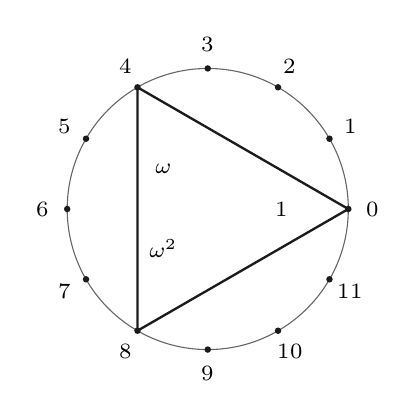
\begin{tikzpicture}[scale=1.02, every node/.style={font=\fontsize{7.9}{9}\selectfont}]
  \draw[mediumink,line width=.4pt] (0,0) circle (1.75);
  \draw[ink,line width=.85pt] (0:1.75)--(120:1.75)--(240:1.75)--cycle;
  \foreach \k in {0,...,11}{
    \pgfmathsetmacro{\a}{30*\k}
    \fill[ink] (\a:1.75) circle (1.15pt);
    \node at (\a:2.05) {$\k$};
  }
  \node at (0:.92) {$1$};
  \node at (138:.74) {$\omega$};
  \node at (222:.74) {$\omega^2$};
\end{tikzpicture}
\vspace{0.5mm}
\begin{minipage}{\linewidth}\centering
{\fontsize{8.8}{11}\selectfont Vertices indexed by $k$; triangle: cube roots.\par}
\end{minipage}
\end{column}
\end{columns}
\end{frame}

% 8 — table displays the valuation calculation cleanly.
\begin{frame}[t]{Counting multiplicities.}
\tightbody
At each twelfth root $\zeta_k=e^{ik\pi/6}$, compare the multiplicities on both sides of Eq.~\eqref{eq:geometric-product}. Multiplicities add under multiplication:
\begin{center}
\renewcommand{\arraystretch}{1.05}
\fontsize{9.25}{11.1}\selectfont
\begin{tabular}{@{}llccc@{}}
\toprule
 & & \multicolumn{3}{c}{Multiplicity in}\tabularnewline
\cmidrule(l){3-5}
Root & $k$ & $(1-x^3)(1-x^{12})$ & $(1-x)(1-x^4)$ & $P(x)$\\
\midrule
$1$ & $0$ & $2$ & $2$ & $0$\\
$i,-1,-i$ & $3,6,9$ & $1$ & $1$ & $0$\\
$\omega,\omega^2$ & $4,8$ & $2$ & $0$ & $\mathbf 2$\\
The other six & $1,2,5,7,10,11$ & $1$ & $0$ & $1$\\
\bottomrule
\end{tabular}
\end{center}
The roots $\omega$ and $\omega^2$ are double, the other six are simple, and $1$, $i$, $-1$ and $-i$ are excluded. This accounts for all ten roots, counted with multiplicity.
\end{frame}

% 9 — full vector diagram of roots and exclusions.
\begin{frame}[t]{The roots on the unit circle.}
\slidebody
\begin{columns}[T,onlytextwidth]
\begin{column}{.43\textwidth}
\centering
\vspace{1.8mm}
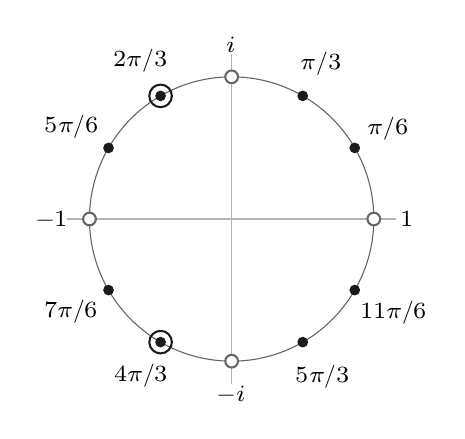
\begin{tikzpicture}[scale=1.02, every node/.style={font=\fontsize{8.4}{10}\selectfont}]
 \draw[softink,line width=.4pt] (-2.05,0)--(2.05,0);
 \draw[softink,line width=.4pt] (0,-2.05)--(0,2.05);
 \draw[mediumink,line width=.4pt] (0,0) circle (1.77);
 \foreach \k in {0,...,11}{
   \pgfmathsetmacro{\a}{30*\k}
   \ifnum\k=0 \draw[mediumink,fill=white,line width=.75pt] (\a:1.77) circle (2.25pt);
   \else\ifnum\k=3 \draw[mediumink,fill=white,line width=.75pt] (\a:1.77) circle (2.25pt);
   \else\ifnum\k=6 \draw[mediumink,fill=white,line width=.75pt] (\a:1.77) circle (2.25pt);
   \else\ifnum\k=9 \draw[mediumink,fill=white,line width=.75pt] (\a:1.77) circle (2.25pt);
   \else\fill[ink] (\a:1.77) circle (1.9pt);
     \ifnum\k=4 \draw[ink,line width=.75pt] (\a:1.77) circle (4pt);\fi
     \ifnum\k=8 \draw[ink,line width=.75pt] (\a:1.77) circle (4pt);\fi
   \fi\fi\fi\fi
 }
 \node at (0:2.18) {$1$}; \node at (180:2.23) {$-1$};
 \node at (90:2.17) {$i$}; \node at (270:2.18) {$-i$};
 \node at (30:2.25) {$\pi/6$}; \node at (60:2.23) {$\pi/3$};
 \node at (120:2.27) {$2\pi/3$}; \node at (150:2.3) {$5\pi/6$};
 \node at (210:2.31) {$7\pi/6$}; \node at (240:2.25) {$4\pi/3$};
 \node at (300:2.27) {$5\pi/3$}; \node at (330:2.33) {$11\pi/6$};
\end{tikzpicture}
\end{column}
\begin{column}{.56\textwidth}
Writing $x=e^{i\theta}$, the six simple roots occur at
\begin{equation}\label{eq:simple-angles}
\smallequation
\theta\in\left\{\frac{\pi}{6},\frac{\pi}{3},\frac{5\pi}{6},
\frac{7\pi}{6},\frac{5\pi}{3},\frac{11\pi}{6}\right\}.
\end{equation}
The two double roots occur at
\begin{equation}\label{eq:double-angles}
\theta\in\left\{\frac{2\pi}{3},\frac{4\pi}{3}\right\},
\qquad x\in\{\omega,\omega^2\}.
\end{equation}
\simplemark\ Simple;\quad \dblmark\ double;\quad \excludedmark\ not a root. Since $P$ has real coefficients, all non-real roots occur in conjugate pairs with equal multiplicity, as the symmetry of the diagram confirms.
\end{column}
\end{columns}
\end{frame}

% 10 — original independent fourth-root derivation, retained as verification.
\begin{frame}[t]{Check: the substitution $t=x^4$.}
\tightbody
\fontsize{9.9}{11.2}\selectfont\setlength{\parskip}{2pt}
The substitution $t=x^4$ provides an independent check. Solving its quadratic equation gives
\begin{equation}\label{eq:check-t}
  t=\frac{-1\pm i\sqrt{3}}{2}=e^{\pm2\pi i/3}.
\end{equation}
Taking the fourth roots of $x^4=t$ produces the two angular families
\begin{equation}\label{eq:check-general}
  \theta=\pm\frac{\pi}{6}+\frac{k\pi}{2},\qquad k=0,1,2,3,
\end{equation}
which, after reduction modulo $2\pi$, become
\begin{equation}\label{eq:check-angles}
\begin{aligned}
 \theta_+&\in\left\{\frac{\pi}{6},\frac{2\pi}{3},\frac{7\pi}{6},\frac{5\pi}{3}\right\},\\
 \theta_-&\in\left\{\frac{11\pi}{6},\frac{\pi}{3},\frac{5\pi}{6},\frac{4\pi}{3}\right\}.
\end{aligned}
\end{equation}
The roots $\omega$ and $\omega^2$ occur in both factors and are therefore double.
\end{frame}

% 11 — real factors from conjugate roots.
\begin{frame}[t]{Factorization over the real numbers.}
\slidebody
Since $P$ has real coefficients, every non-real zero $e^{i\theta}$ is accompanied by its complex conjugate $e^{-i\theta}$. The pair determines a quadratic polynomial with real coefficients:
\begin{equation}\label{eq:real-quadratic}
 (x-e^{i\theta})(x-e^{-i\theta})=x^2-2x\cos\theta+1.
\end{equation}
The four conjugate pairs have angles $2\pi/3$, $\pi/3$, $\pi/6$, and $5\pi/6$. Including the multiplicity of the cube roots gives
\begin{equation}\label{eq:real-factor}
\smallequation
\begin{aligned}
P(x)={}&(x^2+x+1)^2(x^2-x+1)\\
&\times(x^2-\sqrt{3}\,x+1)(x^2+\sqrt{3}\,x+1).
\end{aligned}
\end{equation}
Each quadratic factor has discriminant $4\cos^2\theta-4=-4\sin^2\theta<0$, because none of the four angles equals $0$ or $\pi$. Thus the displayed factors are irreducible over $\mathbb R$ and $P$ has no real zeros.
\end{frame}

% 12 — rational coefficient factors and merging of radical terms.
\begin{frame}[t]{Factorization over the rational numbers.}
\slidebody
The two factors containing $\sqrt{3}$ have real coefficients but do not individually have rational coefficients. Their product eliminates the irrational terms:
\begin{equation}\label{eq:rational-merge}
 (x^2-\sqrt{3}\,x+1)(x^2+\sqrt{3}\,x+1)=x^4-x^2+1.
\end{equation}
Consequently, the factorization in Eq.~\eqref{eq:real-factor} can be rewritten entirely with rational coefficients:
\begin{equation}\label{eq:rational-factor}
 P(x)=(x^2+x+1)^2(x^2-x+1)(x^4-x^2+1).
\end{equation}
Each factor has leading coefficient $1$: the coefficient multiplying its highest power of $x$ is unity. A polynomial with this property is called \emph{monic}. The factorization above also makes clear that passing from real to rational coefficients changes the grouping of roots into factors, without changing the roots of $P$ or their multiplicities.
\end{frame}

% 13 — careful introduction to cyclotomic polynomials.
\begin{frame}[t]{Monic and cyclotomic polynomials.}
\tightbody
Recall that a polynomial is \emph{monic} if its leading coefficient is $1$; for example, $x^2+x+1$ is monic, whereas $2x^2+x+1$ is not. An $n$-th root of unity is \emph{primitive} if its multiplicative order is exactly $n$, meaning that no smaller positive power equals $1$. The \emph{cyclotomic polynomial} $\Phi_n(x)$ is the monic polynomial whose zeros are precisely the primitive $n$-th roots of unity.

For the orders appearing in this problem, these polynomials are
\begin{equation}\label{eq:phi-explicit}
\begin{aligned}
 \Phi_3(x)&=x^2+x+1,\\
 \Phi_6(x)&=x^2-x+1,\\
 \Phi_{12}(x)&=x^4-x^2+1.
\end{aligned}
\end{equation}
The rational factorization therefore has the concise form
\begin{equation}\label{eq:cyclotomic}
 P(x)=\Phi_3(x)^2\,\Phi_6(x)\,\Phi_{12}(x).
\end{equation}
The squared factor $\Phi_3$ records the double multiplicity of the primitive cube roots of unity.
\end{frame}

% 14 — original conclusion, retained.
\begin{frame}[t]{Conclusion.}
\tightbody
The solutions of Eq.~\eqref{eq:problem}, with their multiplicities, are
\begin{equation}\label{eq:final-roots}
 x=e^{ik\pi/6},\qquad
 k\in\{1,2,4,5,7,8,10,11\},
 \qquad k=4,8\ \text{double}.
\end{equation}
They are the twelfth roots of unity other than $\pm1$ and $\pm i$, with $\omega$ and $\omega^2$ occurring twice. No root is real. The elementary grouping in Eq.~\eqref{eq:ansatz} proves the factorization immediately, while the base-$4$ explanation and the geometric-series identity reveal the regularity behind that algebraic observation and justify the complete multiplicity count.

The construction extends beyond the present example. If $m,b\ge 2$ and $\gcd(m,b)=1$, every $m$-th root of unity other than $1$ is a double root of
\begin{equation}\label{eq:generalization}
 \left(\sum_{r=0}^{m-1}x^r\right)
 \left(\sum_{s=0}^{m-1}x^{bs}\right).
\end{equation}
The problem studied here corresponds to $m=3$ and $b=4$.
\end{frame}

% 15 — original reference slide.
\begin{frame}[t]{References.}
\slidebody
\begingroup
\fontsize{10.45}{14.0}\selectfont
\begin{list}{\textbullet}{%
\setlength{\leftmargin}{5.5mm}%
\setlength{\labelwidth}{2.5mm}%
\setlength{\labelsep}{2.1mm}%
\setlength{\itemindent}{0pt}%
\setlength{\itemsep}{3.8mm}%
\setlength{\parsep}{0pt}%
}
\item \justifying T. Andreescu and D. Andrica, \textit{Complex Numbers from A to \ldots{} Z}, second edition, Birkhäuser, 2014.
\item \justifying E. J. Barbeau, \textit{Polynomials}, Problem Books in Mathematics, Springer, 1989.
\item \justifying D. S. Dummit and R. M. Foote, \textit{Abstract Algebra}, third edition, Wiley, 2004, Sec. 13.6 (cyclotomic polynomials and extensions).
\item \justifying T. Needham, \textit{Visual Complex Analysis}, Oxford University Press, 1997.
\end{list}
\endgroup
\end{frame}
\end{document}